\newpage
\subsection{Diseño}

Al unir todos los componentes antes mencionados se obtiene el circuito mostrado en la figura \ref{circuito_final}.\\
De izquierda a derecha primero se encuentran 2 pulsadores los cuales son los botones peatonales A y B; estos en paralelo de modo que pueden ser activados en cualquier dirección e independientemente de cuál se accione, los dos podrían empezar la secuencia del cambio de estado. Seguidamente se encuentra la lógica para el control de rebote que se explicará posteriormente. Se utiliza el pin D3 como entrada del MCU el cual recibirá la señal de los botones y, a la salida, los pines B3, B2, B1 y B0. En total 4 pines para accionar dos luces por semáforo. B3 y B2 se encargan de encender la luz roja y verde del semáforo de peatones respectivamente. Para los peatones hay dos semáforos en paralelo; en total 4 LEDs. Los pines B1 y B0 se encargan de encender la luz roja y luz verde del paso vehicular respectivamente. Por último se encuentran los resistores de control de corriente para los LEDs y al final del circuito se encuentran los propios LEDs.

\begin{figure}[H]
\centering
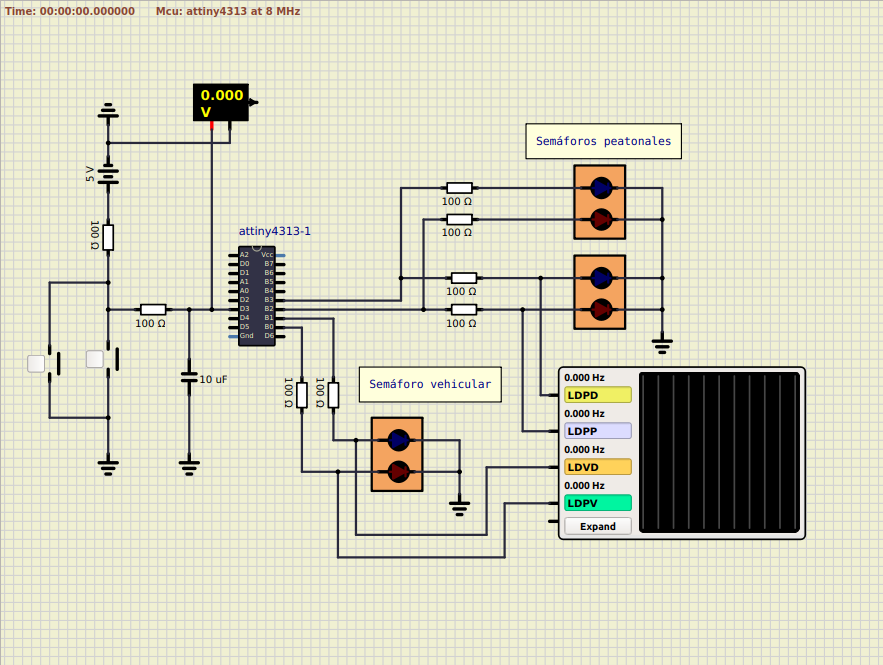
\includegraphics[scale=0.7]{./images/semaforo_circuito.png}
\caption{Diseño completo final (Autoría propia).}
\label{circuito_final}
\end{figure}

\subsubsection{Rebote del pulsador}

Cuando se presiona un pulsador, la salida del mismo no es una señal totalmente limpia, sino que presenta rebotes. Esto se debe a que los contactos del pulsador suelen presentar un pequeño rebote entre ellos. Esto representa un inconveniente ya que los rebotes pueden introducir falsas lecturas al sistema. Para contrarrestar este efecto en el circuito diseñado, se agregó el siguiente filtro pasivo: 

\begin{figure}[H]
    \centering
    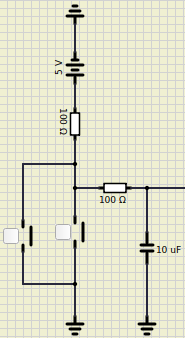
\includegraphics[width=0.275\textwidth]{images/filtro.png}
    \caption{Filtro diseñado para eliminar el efecto del rebote de los pulsadores}
    \label{filtro}
\end{figure}


Tomando en cuenta que la entrada del circuito es DC y, por lo tanto, no es necesario diseñar el filtro para atenuar un rango de frecuencias, se escogieron los valores de los elementos que componen dicho filtro arbitrariamente. Así que tomando un capacitor de $100\,pF$ junto con dos resistencias, cada una de $100\,\Omega$, se tiene que la constante de carga de este filtro sería:

\begin{equation}
    \tau = R \cdot C = 200\,\Omega \cdot 100\,pF = 20\,ns
\end{equation}

El periodo de tiempo obtenido es lo suficientemente grande como para eliminar cualquier distorsión en la señal de entrada, producido por el rebote, pero también es lo bastante pequeño como para que su efecto sea imperceptible por el usuario.

\subsubsection{Resistores}

Para controlar la corriente en los LEDs de modo que no fuere tan alta como para quemarlos ni tan pequeña como para una iluminación, se parte de que para su funcionamiento ideal esta debería ser en directo como máximo $20 mA$. Los mismos tienen una caída en directo que va desde $2.2V$ hasta $3V$. Para tener seguridad se toma el valor máximo de tensión posible. Realizando la malla (Asumiendo $5V$ ideales a la salida del mcu):
\[
-5V+V_R+3V = 0
\]
\[
\rightarrow V_R = 2V
\]

Para asegurar esto en el caso de corriente máxima:

\[
I = \frac{V}{R}
\]
\[
20mA = \frac{2}{R}
\]
\[
\rightarrow R = \frac{2}{20mA} = 100 \Omega
\]